\documentclass[11pt,openright,twoside,a4paper]{report}

% These are the includes required for the doc 
%% Package to includes to provide additional functionality to the dissertation document
\usepackage{harvard}    	% Uses harvard style referencing
\usepackage{graphicx}   	% Permits import of various graphics formats
\usepackage{multicol}   	% Provides ability to split output into columns
\usepackage{listings}   	% Provides styled code listings
\usepackage{minted}         % Minted theme for code listings
\usepackage{xcolor}         % Set background colours for code listings
\usepackage{float}      	% Suppresses floating for tables and figures when using "H"
\usepackage{etoolbox}   	% enable bibliography to be added to the table of contents
\usepackage{comment}    	% enable block of comments
\usepackage{enumitem}       % resume enumerations
\usepackage{breakurl}       % used to break long url links
\usepackage{longtable}      % span tables through multiple pages. Note: It may be necessary to compile the document several times to get a multi-page table to line up properly
\usepackage[breaklinks]{hyperref}   % Provides hyperlinks to sections automatically
\usepackage[export]{adjustbox}      % allows figures to be positioned (left-center-right)

\usepackage[english]{babel}
\usepackage[utf8]{inputenc}

%% Set some page size changes from the standard article class
\usepackage[inner=4cm,outer=4cm]{geometry}

%% Format definitions for the style
\bibliographystyle{agsm} %{alpha}
\citationstyle{dcu}
\pagestyle{headings}
\fussy

%% Break long urls with the following characters
\def\UrlBreaks{\do\/\do-\do.\do0}

%% Light grey background colour for code listings
\definecolor{LightGray}{gray}{0.9}

%% Definitions to provide layout in the dissertation title pages
\newenvironment{spaced}[1]
  {\begin{minipage}[c]{\textwidth}\vspace{#1}}
  {\end{minipage}}
\newenvironment{centrespaced}[2]
  {\begin{center}\begin{minipage}[c]{#1}\vspace{#2}}
  {\end{minipage}\end{center}}

%% Copyright page
\newcommand{\declaration}[2]{
  \thispagestyle{empty}
  \begin{spaced}{4em}
    \begin{center}
      \LARGE\textbf{#1}
    \end{center}
  \end{spaced}
  \begin{spaced}{3em}
    \begin{center}
      Submitted by: #2
    \end{center}
  \end{spaced}
  \begin{spaced}{5em}
    \section*{COPYRIGHT}

    Attention is drawn to the fact that copyright of this dissertation rests
    with its author. The Intellectual Property Rights of the products
    produced as part of the project belong to the author unless otherwise specified
    below, in accordance with the University of Bath's policy on intellectual property 
   (see \url{http://www.bath.ac.uk/ordinances/22.pdf}).

    This copy of the dissertation has been supplied on condition that anyone
    who consults it is understood to recognise that its copyright rests with its
    author and that no quotation from the dissertation and no information
    derived from it may be published without the prior written consent of
    the author.

    \section*{Declaration}
    This dissertation is submitted to the University of Bath in accordance
    with the requirements of the degree of Bachelor of Science in the
    Department of Computer Science. No portion of the work in this dissertation
    has been submitted in support of an application for any other degree
    or qualification of this or any other university or institution of learning.
    Except where specifically acknowledged, it is the work of the author.
  \end{spaced}

  \begin{spaced}{5em}
    Signed:
  \end{spaced}
  }


\newcommand{\consultation}[1]{%
\thispagestyle{empty}
\begin{centrespaced}{0.8\textwidth}{0.4\textheight}
\ifnum #1 = 0
This dissertation may be made available for consultation within the
University Library and may be photocopied or lent to other libraries
for the purposes of consultation.
\else
This dissertation may not be consulted, photocopied or lent to other
libraries without the permission of the author for #1 
\ifnum #1 = 1
year
\else
years
\fi
from the date of submission of the dissertation.
\fi
\vspace{4em}

Signed:
\end{centrespaced}
}

\title{Content-based Video Retrieval for Pattern Matching Video Clips}
\author{Adam Jaamour}
\date{Bachelor of Science in Computer Science with Honours\\The University of Bath\\May 2019}

\begin{document}

\setcounter{page}{0}
\pagenumbering{roman}

\maketitle
\newpage

% Set this to the number of years consultation prohibition, or 0 if no limit
\consultation{0}
\newpage

\declaration{Content-based Video Retrieval for Pattern Matching Video Clips}{Adam Jaamour}
\newpage

\abstract
Your abstract should appear here.  An abstract is a short
paragraph describing the aims of the project, what was
achieved and what contributions it has made.
\newpage

\tableofcontents
\newpage
\listoffigures
\newpage
\listoftables
\newpage

\chapter*{Acknowledgements}
Add any acknowledgements here.
\newpage

\setcounter{page}{1}
\pagenumbering{arabic}

\chapter{Introduction}
Add intro here
% \section{Motivation}

During the past decade, the amount of data in the world has grown at exponential rates and is currently showing no signs of slowing down. According to infographics released by IBM, already 2.7 ZB\footnote{Zettabytes. 1 Zb = 1 trillion Gb.} of data existed in the world in 2012 \cite{karr_2012}, enough to fill up almost 40 billion 64 Gb iPhones. This number has since then risen to 8 Zb in 2015 and is expected to reach a shocking yearly production of 35 Zb by 2020 \cite{deutscher_2012} \cite{karr_2012}. 85\% of all the world data is considered to be unstructured data \cite{blumberg2003problem}, which is mainly be made up of multimedia in the form of images and videos.\\

An important factor in this growth is the rise of mobile devices usage and social media. Indeed, the amount of mobile-dependant users has grown at impressive rates, with now 95\% of the United States citizens owning a mobile phone \cite{fanning2012increasing}. People tend to use their mobile devices for most day-to-day activities, with a majority of this time spent on social media services such as YouTube or Facebook. These social networks are one of the primary causes for the exponential growth of unstructured data mentioned earlier, with an average of over 300 hours of new video content constantly uploaded to YouTube every minute. The combination of mobile devices usage and social media data generation are the main contributors in today's flood of unstructured data.\\

Various systems, including commercialised mobile applications, already exist to help organise this unstructured data and render it useful and accessible. These systems already cover specific types of unstructured data such as music, images and CCTV security footage. However, none tackle the problem of unstructured data concerning long videos such as movies. Indeed, with 5,626,984 movies as of December 2018 \cite{imdb2018stats}, a lot of data generated around these movies, e.g. in the form of short recordings or copies circulating on the web, corresponds to unstructured data. Therefore, the goal of this project is to tackle this problem by creating a system targeting long videos that could contribute to improving this ongoing problem.

%%%%%%%%%%%%%%%%%%%%%%%%%%%%%%%%%%%%%%%%%%%%%%%%%%%%%%%%%%%%%%%%%%%%%%%%%%%%%%%%%%

\section{Problem Description}
\label{sec:problem-description}

Content-based video retrieval, or CBVR, is a computer vision task aimed at solving the problem of searching large databases of videos, where ``content'' corresponds to visual information from a video such as colours, shapes or motion that can be extracted and used to retrieve the desired video from a large database efficiently. The main difficulty with content-based video retrieval lies with the reference database of videos itself. As mentioned earlier, the videos in a database correspond to unstructured data, meaning that only the video data\footnote{Video data includes the video frames and the audio.} and its metadata\footnote{Examples of metadata related to a video file includes captions, file name, file type, video length, file size.} are stored in the database. The computations involved in querying a database of videos using only the metadata available and not the visual information from a video itself would be too expensive and slow to compute, but most importantly, highly inefficient \cite{patel2012}. Therefore, analysing the content from video files is a necessity in order to find adequate solutions to the CBVR problem. Another difficulty involves the large size of the database itself. Indeed, more complications arise from databases populated with a large number of videos, especially if their duration is lengthy, e.g. feature-length films. Solutions to those problems hence require intelligent and efficient pattern matching algorithms to overcome the specified difficulties. This is where visual search and the variety of fields it includes such as artificial intelligence, machine learning and database management come in.\\

Several visual search techniques exist for querying databases of unstructured data such as video or image files. These techniques can be classified based on the type of query and on the type of database used, as shown in table \ref{table:visual_search_table}. The most common forms of visual search consist in querying a database of images either with an image (I2I) or with a video (V2I), as depicted in section \ref{sec:v2v_applications} where similar existing systems are mentioned. Another less common variant consists of querying a database of images with a video query (V2I) \cite{araujo2017i2v}. However, this dissertation will solely focus on querying a database of videos with a video query (V2V). Because algorithms from other variants of visual search can be relevant to V2V, existing solutions for these variants will also be explored to find ways potential techniques that could be implemented with this project.\\

% table
\begin{table}[H]
\centering
\begin{tabular}{c|c|c|}
\hline
\multicolumn{1}{|c|}{Image Query} & I2I                & I2V                \\ \hline
\multicolumn{1}{|c|}{Video Query} & V2I                & V2V                \\ \hline
\multicolumn{1}{l|}{}             & Database of Images & Database of Videos \\ \cline{2-3} 
\end{tabular}
\caption{The four types of visual search involving images and videos, classified by type of query used and by type of database being queried.}
\label{table:visual_search_table}
\end{table}

To pattern match the query video to a video in the database, key visual elements from the query video, called \textit{``features''}, are extracted and compared to the same extracted features from videos in the database to find similarities between them. These features can include elements such as colours or object shapes and their motion \cite{patel2012}, as well colour distributions, colour layouts or textures \cite{petkovic2000}, or other unique features such as on-screen text or audio components, e.g. soundtracks, dialogues or sound effects. A broad spectrum of systems exists to efficiently retrieve information from large databases, which are discussed in the section below.

%%%%%%%%%%%%%%%%%%%%%%%%%%%%%%%%%%%%%%%%%%%%%%%%%%%%%%%%%%%%%%%%%%%%%%%%%%%%%%%%%%

\section{Related Systems \& Their Applications}
\label{sec:v2v_applications}

Visual search technology has an endless amount of applications in fields such as education, navigation, utilities and security. Some of the systems using this technology have already found their way to commercial applications. For example, YouTube's Content ID system uses visual search, and more precisely V2V, to detect copyright infringements on user-uploaded videos by automatically comparing an uploaded video with a database of protected videos, allowing YouTube to take action against videos infringing copyrights \cite{youtube-content-id-2012}. Another example is Google Lens\footnote{Google Lens: \url{https://lens.google.com/}}, a mobile application that recognises the environment through a mobile device's camera in order to relay information about objects of interest. For instance, if pointing the camera at a landmark, information such as historical facts or opening hours about that location will be displayed, or if pointing it at a WiFi router's label, the mobile device will automatically connect to the network \cite{villaboas-google-lens2017}. Other applications include A9's Amazon Flow\footnote{A9 Visual Search: \url{https://www.a9.com/what-we-do/visual-search.html}} that uses deep-learning based computer vision to power Amazon's search services, as well as Shazam\footnote{Shazam: \url{https://www.shazam.com/gb/company}}, a mobile application that matches short user-recorded sounds with a piece of music.\\

Aside from the commercialised systems stated in the previous paragraph, many visual search applications are yet to be implemented for large-scale use. For example, a system allowing companies to detect all appearances of their logos during television broadcasts, or a system enabling students to find a section of a recorded lecture by using a lecture slide as a query \cite{araujo2017i2v} are possibilities that need to be explored. Research covering content-based video retrieval has also been published in recent years. For instance, Liu et al. \cite{liu2014mobilevideosearch} discuss a concept similar to this project's aims consisting of a mobile visual search system allowing users to discover videos by pointing their phone at a screen. Recently, research in visual search has gained momentum, notably with the annual TRECVID\footnote{Text REtrieval Conference Video Retrieval Evaluation} conference \cite{2018trecvidawad} hosted by the NIST\footnote{National Institute of Standards and Technology}. This conference's goal is to host workshops that focus on information retrieval research, with an emphasis on content-based retrieval of digital videos \cite{trecvid-general}.

%%%%%%%%%%%%%%%%%%%%%%%%%%%%%%%%%%%%%%%%%%%%%%%%%%%%%%%%%%%%%%%%%%%%%%%%%%%%%%%%%%

\section{Project Aims}
\label{sec:introduction-project-aims}

The aim of the project is therefore to explore the possible implementation of a prototype CBVR algorithm with an orientation towards matching mobile-recorded queries to movies. A commercial system for mobile devices that could work with large databases of movies, as seen in Figure \ref{fig:wireframe}, would be ideal but not a realistic target due to the time constraints set by this project. Thus, this project will aim to achieve the following:

\begin{itemize}
    \item Investigate the different feature extraction and comparison methods that can be used to implement an operational CBVR system.
    \item Explore how the combination of these different methods could be used to design a unique functional system that could eventually work with movies.
    \item Develop a system that can be tested with a vast array of queries and a database.
    \item Evaluate the performance of the system with a reasonable testing database size and realistic queries, and eventually with feature-length movies.
    \item Discuss plans for future work and the limitations that such a system would have if it were to be transformed into a marketable mobile application.
\end{itemize}

\begin{figure}[ht]
\centerline{\includegraphics[width=1.15\textwidth]{figures/introduction/system_wireframe.png}}
\caption{\label{fig:wireframe}Wireframe showing the basic high-level concept of an ideal CBVR mobile application for matching movies.}
\end{figure}

%%%%%%%%%%%%%%%%%%%%%%%%%%%%%%%%%%%%%%%%%%%%%%%%%%%%%%%%%%%%%%%%%%%%%%%%%%%%%%%%%%

\section{Report Structure}

\begin{itemize}
    \item \textbf{Introduction}\\
    An overview of the problem description and applications of similar content-based retrieval systems followed by the motivations for this project and the aims to accomplish.
    \item \textbf{Literature \& Technology Survey}\\
    An extensive study of the literature surrounding the topics required to implement the system, including content-based retrieval concepts, visual content extraction and structural video representations.
    \item \textbf{Requirements}\\
    A detailed listing of the different requirements needed to design and implement the system based on the literature survey.
    \item \textbf{Design}\\
    A high-level exploration of potential solutions to meet the previously established requirements and formulate a final solution to implement.
    \item \textbf{Implementation}\\
    A comprehensive examination of the different steps followed to build a system from conception to a functional prototype.
    \item \textbf{Testing \& Evaluation}\\
    A review of the different tests conducted to assess the efficiency of the system and its quality as a whole.
    \item \textbf{Conclusions}\\
    A summary of the accomplished initial project aims, its limitations and plans for future work.
\end{itemize}

\chapter{Literature Survey}
%%%%%%%%%%%%%%%%%%%%%%%%%%%%%%%%%%%%%%%%%%%%%%%%%%%%%%%%%%%%%%%%%%%%%%%%%%%%%%%%%%
% 1 - CONTENT-BASED RETRIEVAL 
%%%%%%%%%%%%%%%%%%%%%%%%%%%%%%%%%%%%%%%%%%%%%%%%%%%%%%%%%%%%%%%%%%%%%%%%%%%%%%%%%%
\section{Content-Based Retrieval}

Content-based retrieval is a type of visual search technique where large databases of either images or videos are queried to find the closest match to a query image or video. Although this project focuses on content-based video retrieval, also referred to as CBVR\footnote{Content-Based Video Retrieval}, image retrieval techniques (CBIR\footnote{Content-Based Image Retrieval}) will be discussed as well due to their relevance in video retrieval.\\

This section will first review the different video retrieval methods and their evolution, starting from text-based retrieval to content-based retrieval, before addressing the various challenges that exist in video retrieval, such as the additional difficulty caused by the temporal aspect of videos compared to images, and the complications of targeting mobile devices for such a system.

% ----------------------------------------------------

\subsection{Video Retrieval Methods}
\label{sec:cbvr-methods}

Drastic advances in video capturing technology have caused important amounts of unstructured data in the form of videos to be produced in recent years. This has lead to a high-demand to develop new efficient solutions for processing this data, with video retrieval being the answer.\\

Throughout the years, video retrieval has improved in parallel with the breakthroughs in video recording devices. Early video retrieval techniques used a text-based approach where the system accepted text input to search the database of videos \cite{lai2015trajectory}, as seen in Figure \ref{fig:text_vs_content_retrieval}.\emph{a}. For example, the user would input the string query \textit{``De Niro"}, which would return all movies in which Robert De Niro starred or \textit{``Coppola"} to find all movies directed by Francis Ford Coppola. Unique aspects of the video clip such as movie credits or sports scores were often analysed using OCR\footnote{Optical Character Recognition} technology \cite{li2002text}. The query text was then compared to a video file's content, such as colours, shapes, texture, luminance or objects, or to the file's metadata\footnote{The data associated to a video file}, such as the video title, author, date, content description, commentaries, captions or keywords \cite{li2002text} \cite{feng2011} \cite{patel2012}. However, these techniques were highly inefficient compared to content-based techniques as they often relied on manually noted annotations and textual descriptions to find similarities for matching the query video to a video in the database and did not make use of the actual visual content that describes a video.\\

\begin{figure}[h]
\centerline{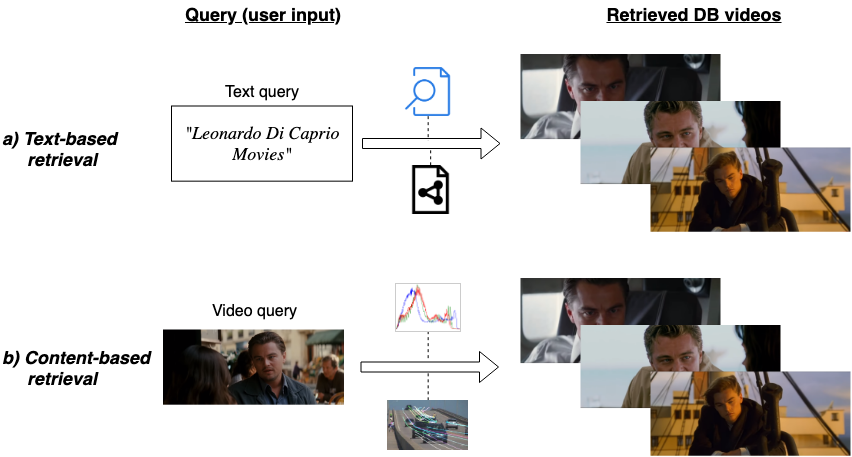
\includegraphics[width=\textwidth]{figures/content_text-retrieval_comparison.png}}
\caption{\label{fig:text_vs_content_retrieval}Illustrations of a text-based content-retrieval system \emph{(a)}, a content-based video retrieval system \emph{(b)}, and the project's desired CBVR system \emph{(c)}.}
\end{figure}

Content-based retrieval techniques quickly replaced text-based retrieval techniques towards the end of the 20th century by making use of the visual content to compute similarities between videos \cite{lai2015trajectory}. Instead of accepting a text string, the system takes a video as input to extract its visual contents, as shown in Figure \ref{fig:text_vs_content_retrieval}.\emph{b}. According to Petković et al. \cite{petkovic2000}, this visual content can be broken down into three different categories:
\begin{itemize}
    \item \textit{Raw data}, which corresponds to individual raw video frames and the video file's attributes such as the frame rate per seconds, the number of bits per pixel or the colour model used.
    \item \textit{Low-level visual content}  consists of the visual features that describe a video. This content includes colours, shapes, textures and motion. Low-level visual content can be extracted into static features such as histograms (see Section \ref{sec:color-based-features}) or dynamic features such as objects or motion (see Section \ref{sec:dynamic-features}) using a wide variety of existing techniques. Once the content has been extracted, it can be used to first compute similarities between videos \cite{lai2015trajectory} and later pattern match them.
    \item \textit{Semantic content} contains the high-level concepts that are present in a video. These high-level concepts can be described as objects or events using the features. To extract semantic content from a video, a grammar of rules for objects must be provided. An example of an object rule could be "if the shape is round, the colour is orange and the object is moving, then that object is a basketball".
\end{itemize}

In comparison to raw data, low-level visual content provides the most relevant visual information that can be extracted from a video for the purpose of a CBVR system. Semantic content extraction adds an additional layer of complexity compared to low-level visual content extraction as it requires domain knowledge and user interaction \cite{petkovic2000}. Therefore, this project will focus on using low-level visual content to extract information about the video and compute the similarities between the query video and database videos. It is important to note that this project's goal differs from classic CBVR systems where a list of videos is returned (see in Figure \ref{fig:text_vs_content_retrieval}.\emph{b}), as it must return a specific video that matches the most the query video. To improve the pattern matching accuracy phase, raw data (e.g. audio) and metadata (e.g. captions) may be used to improve the pattern matching accuracy \cite{patel2012}.\\

% ----------------------------------------------------

\subsection{Temporal Aspects of Videos}
\label{sec:temporal-aspect-videos}

\subsubsection{Temporal Structure of a Video}

The most important difference between content-based image retrieval and video retrieval lies within the temporal aspect of the video. Naturally, the temporal aspect of a video clip stores supplementary information about the content, including dynamic low-level visual content e.g. an object's motion, and semantic content e.g. actions and events. According to A. Araujo et al. \cite{araujo2017i2v}, a video's temporal structure can be subdivided into three units, as shown in Figure \ref{fig:temporal_structure}:
\begin{itemize}
    \item \textit{Frames} correspond to the smallest temporal unit of a video file. A single segment of a video is referred to as a frame. Frames are also used to describe the frame rate (the frequency at which consecutive stills appear on a screen every second) e.g. ``24 fps'' corresponds to a video made up of 24 stills per second.
    \item \textit{Shots} are grouped sequences of visually similar frames. They are usually described  in seconds.
    \item \textit{Scenes} are a collection of shots which are related based on the action and objects present in the shot, thus giving them a semantic aspect. The length of a scene 
    is generally calculated in minutes rather than seconds.
\end{itemize}

\begin{figure}[h]
\centerline{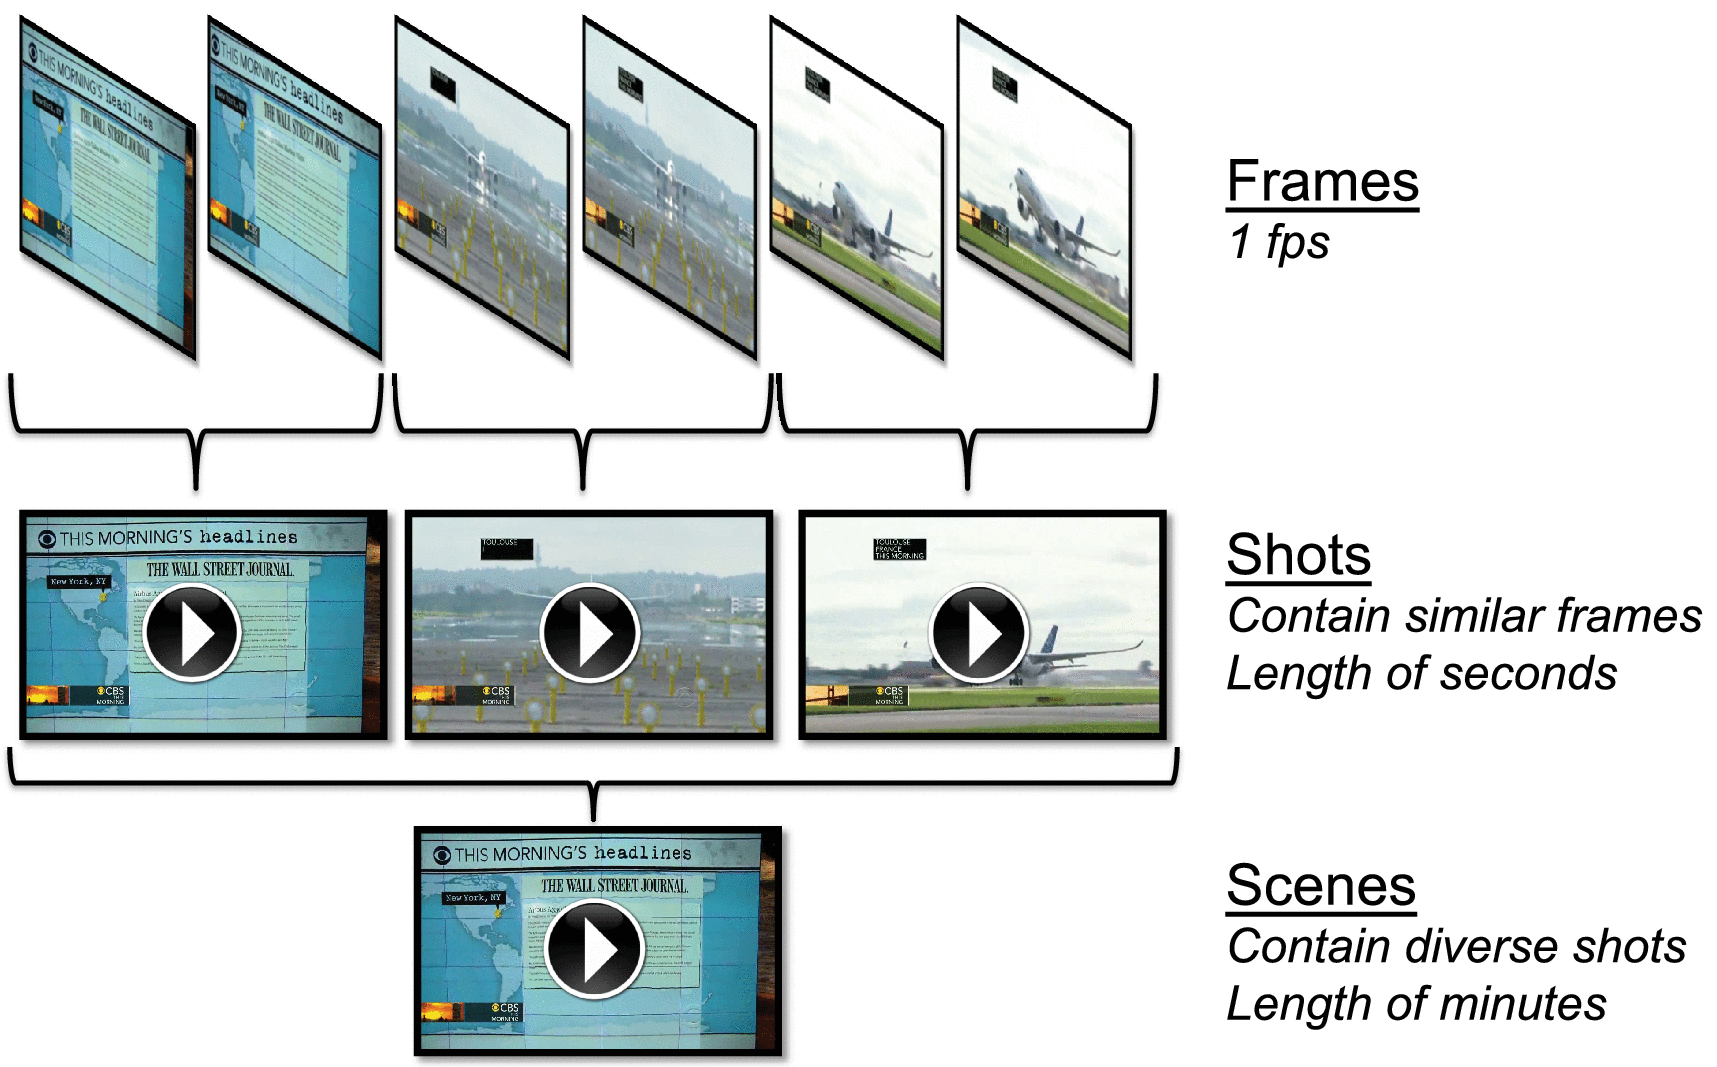
\includegraphics[width=0.75\textwidth]{figures/temporal_structure_videos.png}}
\caption{\label{fig:temporal_structure}Temporal structure of videos, including the different terms used to describe video temporal units. Figure courtesy of A. Araujo et al.}
\end{figure}

Because this project will explore possible solutions to create a CBVR system targeting databases of feature-length movies, a fourth video temporal structure category relevant to this project can be added to Araujo et al.'s initial list:
\begin{itemize}
    \item \textit{Movies} can be described as a large group of scenes that are used to tell a story. Movie durations commonly range from one to three hours.
\end{itemize}

\subsubsection{Challenges of Temporality}

Multiple challenges arise when dealing with CBVR systems in contrast to CBIR systems as the videos' temporal aspect adds a new dimension of complexity when extracting visual information. While the low-level visual content describing images remains mostly the same for videos (see Section ref-section), some new information that did not exist in images can be extracted, such motion. As mentioned previously, videos are a made up of frames, which make up shots when a combination of similar frames are played in succession. This means that videos carry information about motion, such as the trajectory of objects. This introduces unique challenges to the algorithms used to extract motion.\\

Because videos are made up of numerous stills, usually around 24 frames per second \cite{brownlow1980silentfilm}, two consecutive frames are near-identical. The pixels describing an object in one frame will remain the same in the next frame, except for the edge pixels perpendicular to the motion's trajectory \cite{bradski2008opencv}.\\

Figure \ref{fig:forrest_gump_frames} shows six frames from Forrest Gump's famous running shot, which lasts 44 seconds, making up a total of 1056 frames. Each frame in the figure was captured with 10-second intervals, meaning 240 frames separate each still. In the first three frames, the group of people running in the background barely moves in the space of 20 seconds. The pixels that describe the group in the shot remain mostly unchanged for all of the frames between the 3 samples, equivalent to 480 frames, with a few additional pixels describing the group as it advances towards the camera. The same can be said about the red cap in the last two frames. Most of the pixels making up the cap in the fifth frame remain the same in the sixth frame. This example perfectly betrays the reason why analysing a video frame by frame would be extremely inefficient when it comes to CBVR. Due to the similarities between consecutive frames, these should be aggregated \cite{araujo2017i2v} to describe a shot by using a selection of frames, such as taking the six frames in Figure \ref{fig:forrest_gump_frames} to describe the entire 44 seconds of video, rather than keeping the original 1056 frames to describe it.

\begin{figure}[h]
\centerline{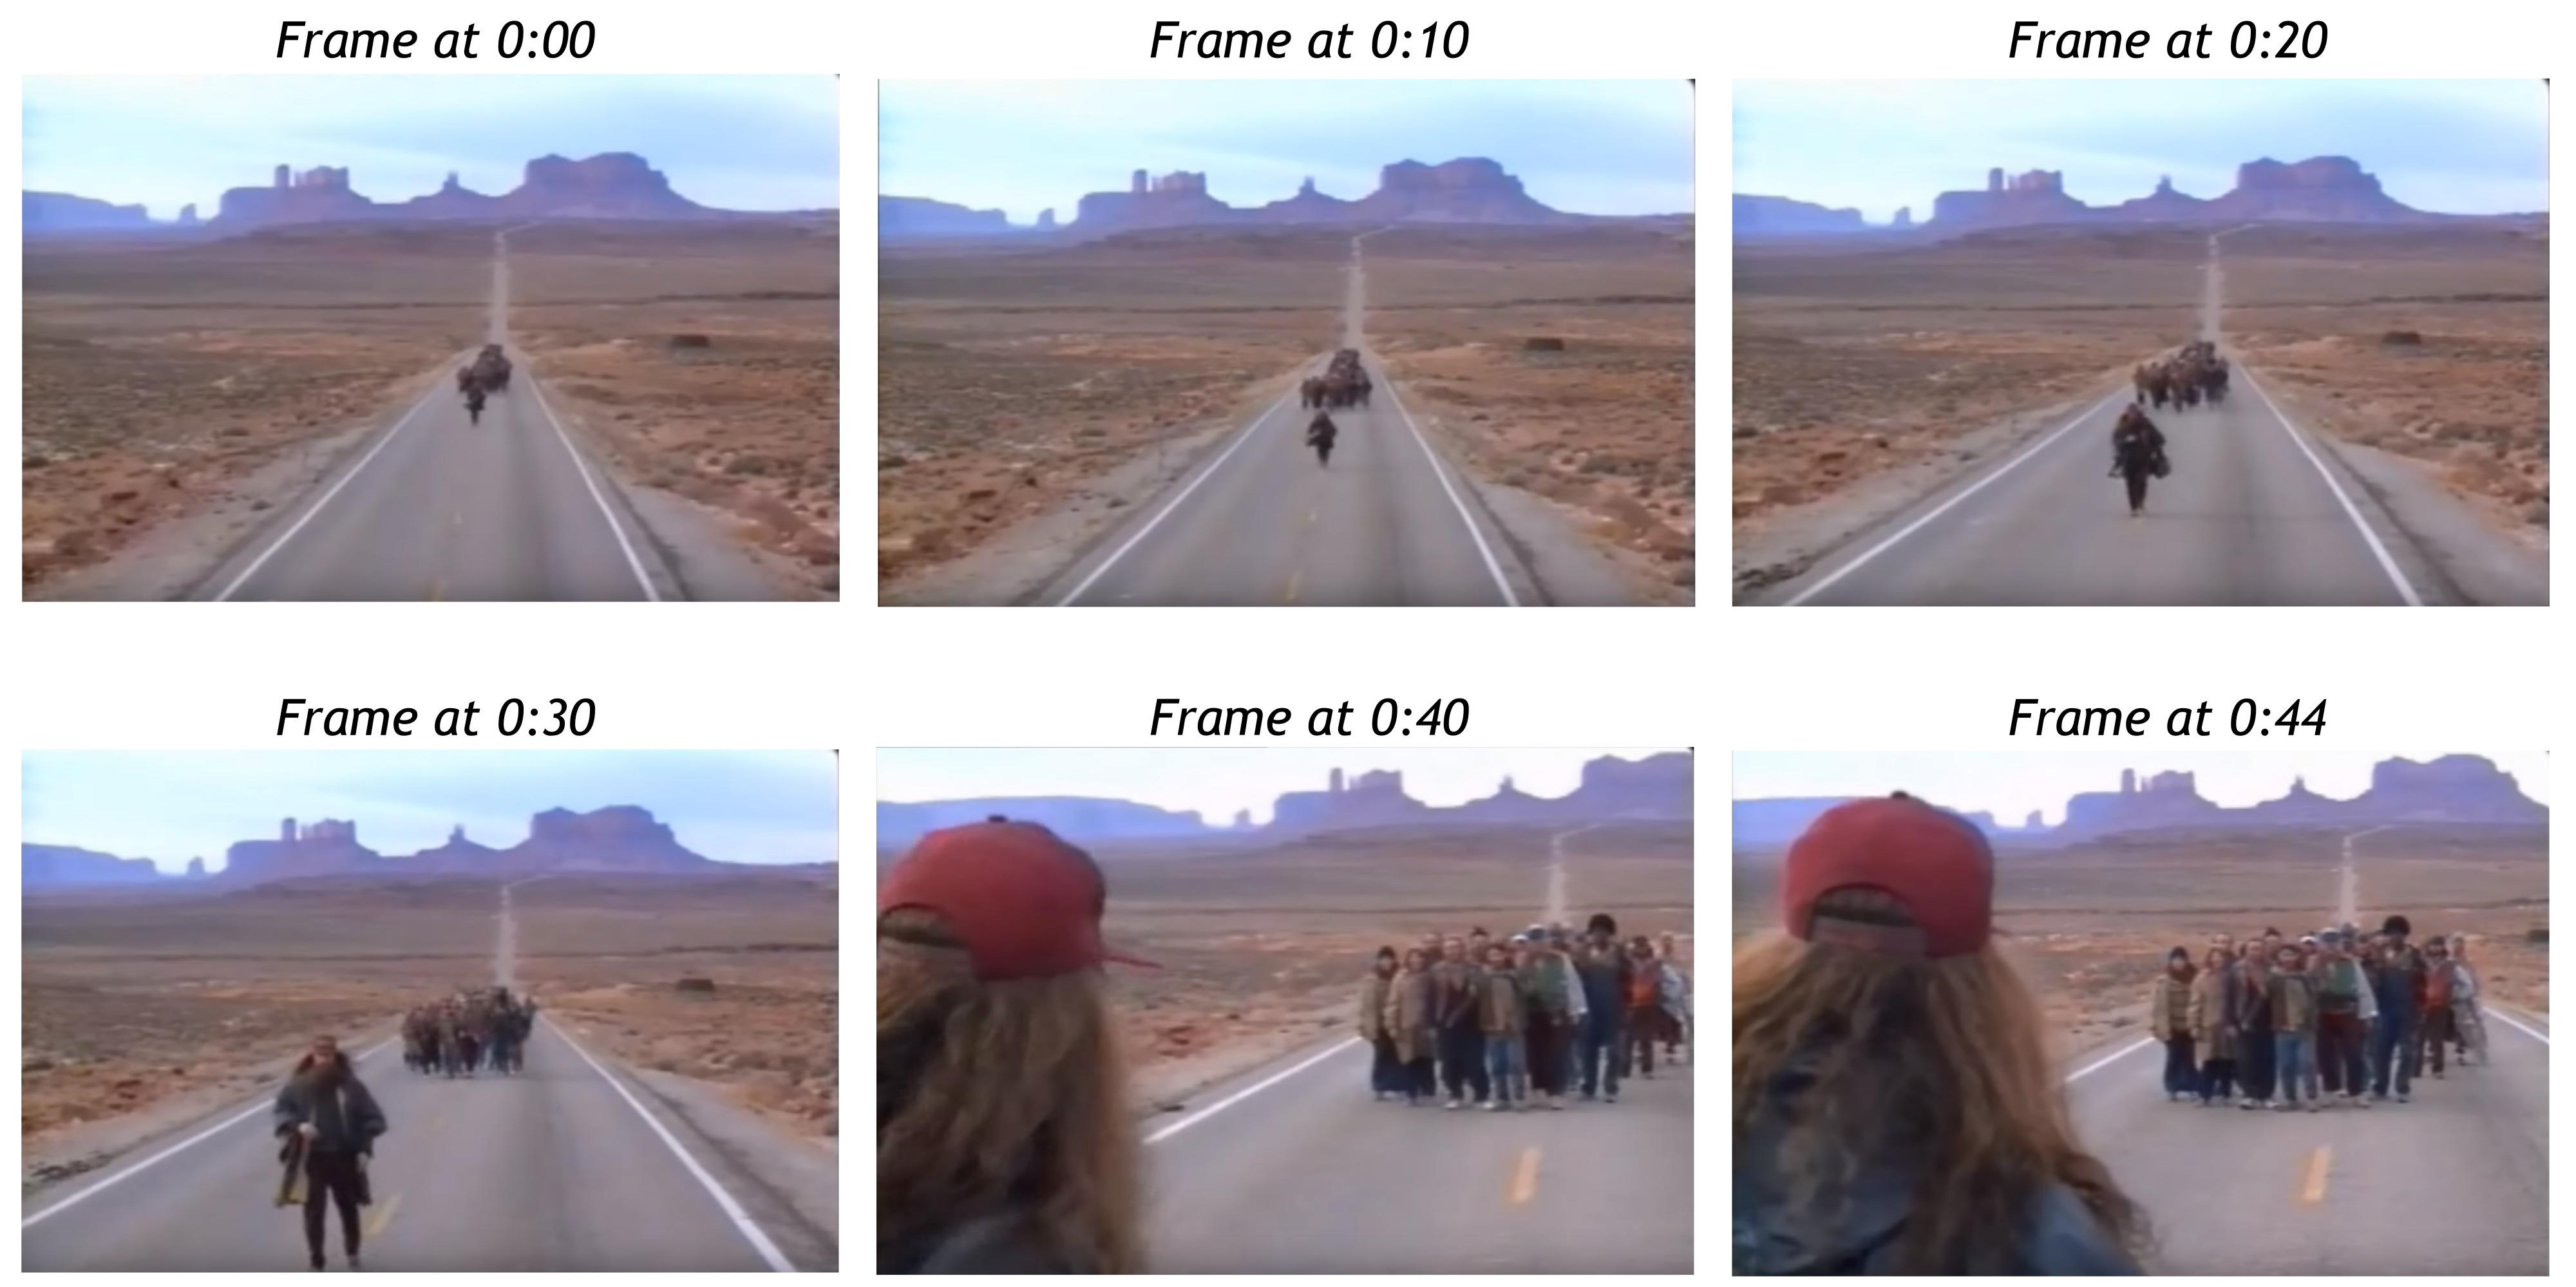
\includegraphics[width=\textwidth]{figures/forrest_gump_shot.jpg}}
\caption{\label{fig:forrest_gump_frames}Frames from the famous running scene in Forrest Gump extracted at intervals of 10 seconds. Video frames courtesy of \textit{``Forrest Gump long run scene"} YouTube video available online: \url{https://youtu.be/QgnJ8GpsBG8?t=325}.}
\end{figure}

\begin{comment}
    On top project aim mobile device using a database of feature-length movies.\\
    \cite{araujo2017i2v}One of the problems regarding video retrieval is the temporal aspect of the data. A solution to overcome the temporal aspect of the data is to aggregate each video into a compact signature to allow quicker and more efficient matching (when matching the query video to a video in the database).\\ 
    temporal aggregation problem of videos compared to images
\end{comment}

% ----------------------------------------------------

\subsection{CBVR for Mobile Devices}

The aforementioned project aim is for the system to work on mobile devices for two reasons. The first reason, as shown in Figure \ref{fig:wireframe} is to allow users to directly use their mobile phone to record the query video by pointing their camera to a screen displaying a movie, which will in turn tell them which movie is being played. Additional information retrieved from IMDb\footnote{Internet Movie Database}, such as cast, crew, ratings, runtime and synopsis could also be displayed. The second reason is the popularity of mobile devices, which may be due to the improvements made on mobile phones' processing power, allowing more tasks to be carried out through this medium. However, such a system on a mobile device causes many problems regarding the query video recording method and the computational power available on mobile devices.\\

\begin{figure}[h]
\centerline{\includegraphics[width=1.15\textwidth]{figures/system_wireframe.png}}
\caption{\label{fig:wireframe}Wireframe showing the basic high-level concept of the system.}
\end{figure}

\subsubsection{Query Video Quality}

Large visual differences are caused between the query clip and the actual clip stored in the database due to the capture conditions \cite{liu2014mobilevideosearch} \cite{wang2016actionregonition} such as:
\begin{itemize}
    \item Undesired camera movements due to unstable recording e.g. unstable recording, hand shaking.
    \item Low-quality recording due to poor user recording e.g. scaling and rotation, and due to the environment conditions e.g. lighting, reflections, blurring.
    \item Video noise because of the camera sensor.
    \item Decoding artefacts causes by various file compression.
\end{itemize}

These low-quality conditions add difficulty to the pattern matching phase where the similarities between the query video and database videos have to be computed. Indeed, if the query video is very different to the actual video, then the noisy elements of the video query must filtered out. For example, if the recorded video is shaky, then this shaking motion has to be pruned before analysing the recorded clip's motion. However, processing power must be used from the actual visual content extraction and pattern matching phases to be used for video noise filtering.

\subsubsection{User Experience}

According to Liu et al. \cite{liu2014mobilevideosearch}, the majority of mobile device users expect a polished product with quick video query and instant or progressive results, meaning that the searching algorithms must be efficient. However, one of the downsides of mobile devices is the computation power constraints. Despite the improvements of mobile processors, desktop devices still remain more powerful than mobile ones. A solution that Liu et al. suggest is to retrieve the low-level visual content locally on the mobile device, and send the query to a server where the pattern matching will take place \cite{liu2014mobilevideosearch}. This allows heavy computations to be off-loaded from the mobile device. Once a match is found, the result is returned to the user on his mobile device. A downside to this approach is the new constraint on network bandwidth rather than computational power.

\begin{comment}
    % todo - spread in sections above
    \subsubsection{Computational efficiency and database size}
    
    At the early stages of the development phase of the project, the database of videos for the system will be made up of shots only, lasting on average ten seconds. Longer videos will be used progressively based on the system's progress with shorter videos.\\
    mention \cite{hanjalic1999moviesegmentation}
    
    \cite{wang2016actionregonition}
    A challenge also lies within the computational power needed to process all the data in a database efficiently.\\
\end{comment}


%%%%%%%%%%%%%%%%%%%%%%%%%%%%%%%%%%%%%%%%%%%%%%%%%%%%%%%%%%%%%%%%%%%%%%%%%%%%%%%%%%
% 2 - VISUAL CONTENT EXTRACTION FOR PATTERN MATCHING VIDEOS
%%%%%%%%%%%%%%%%%%%%%%%%%%%%%%%%%%%%%%%%%%%%%%%%%%%%%%%%%%%%%%%%%%%%%%%%%%%%%%%%%%
\section{Visual Content Extraction for Pattern Matching Videos}
\label{sec:visual-content-extraction}

Extracting the visual content from a video allows this content to be used to describe videos and compute similarities between them. This visual content is extracted from the aforementioned low-level visual content (see Section \ref{sec:cbvr-methods}) \cite{petkovic2000} and stored in the form features, also referred to as visual descriptors. The term ``features'' is very broad and can be used to describe many different visual aspects in an image or in a video, ranging from colours, shapes and textures to points, edges, objects and motion.\\

These features can be divided into two categories: static features and dynamic features \cite{petkovic2000}. This section will first survey examples of static visual descriptors and methods to extract them from videos, and will then focus on examples and methods of extracting dynamic visual descriptors from videos.

% ----------------------------------------------------

\subsection{Static Features}

Methods to extract static features operate on stills, which can correspond to individual video frames, thumbnails or key frames. This means that traditional image techniques can be applied on those stills \cite{hu2011survey}. They are organised in three different categories: colour-based features, texture-based features and shape-based features.

\subsubsection{Colour-based Features}
\label{sec:color-based-features}

The main colour-based features model are colour histograms. In general, a histogram consists of counts of some underlying data that is organised into predetermined bins to a statistical representation of the distribution of that data. Figure \ref{fig:histogram-general-example} depicts an example of a histogram where a collection of points is organised into specific ore-defined bins based on their location relative to a vertical grid.

\begin{figure}[h]
\centerline{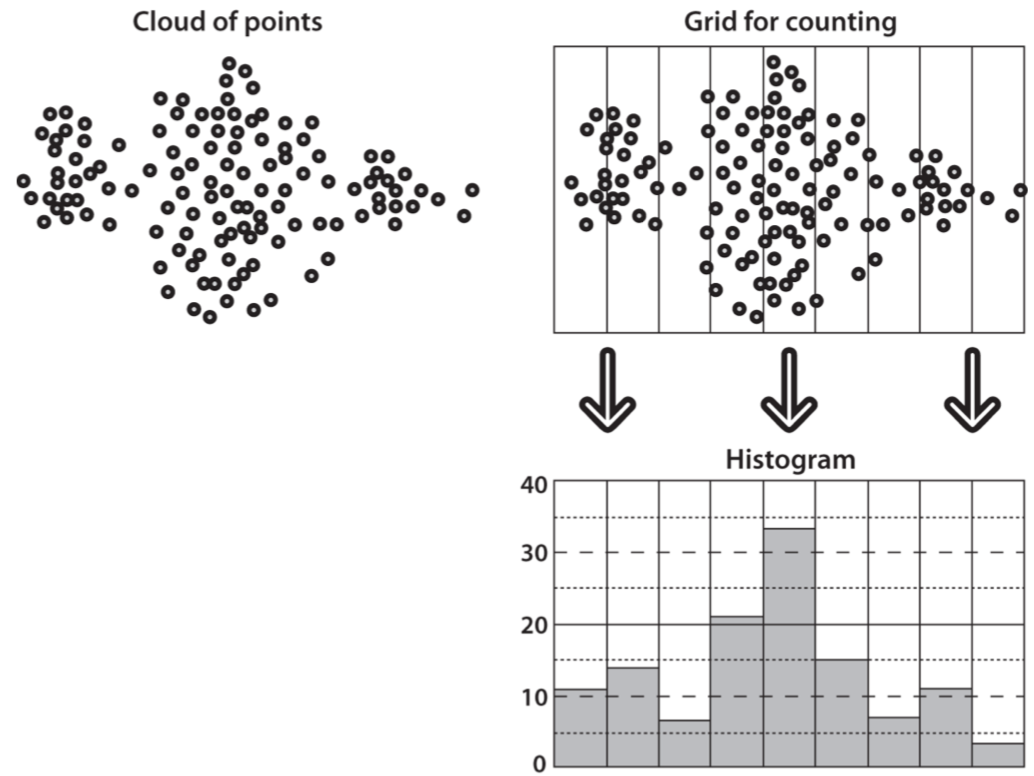
\includegraphics[width=0.70\textwidth]{figures/histogram_general_example.png}}
\caption{\label{fig:histogram-general-example}Example of a histogram counting the location of points relative to a vertical grid. Image courtesy of Bradski and Kaehler.}
\end{figure}

In the case of a colour histogram, the underlying data that the histogram is trying to represent is the distribution of the colour pixels throughout an image or a video frame. Different kinds of colour histograms exist as they depend on the chosen colour space, which include RGB\footnote{Red Green Blue}, HSV\footnote{Hue Saturation Value}, HSL\footnote{Hue Saturation Light} or YPbPr colour spaces to name a few. These may vary based on the applications of the colour histograms.\\

Typically, for a RGB colour histogram, 256 bins are used to accurately represent all the possible values that the pixels can take (ranging from 0 to 255) for each of the three RGB channels, which are then plotted as three individual graphs. Choosing the right range for the histogram's bins is crucial to represented the distribution efficiently. If the range of pixels that defined the bins is wider, meaning there are less overall bins, then the histogram's distribution would be too coarse-grained and the general structure of the histogram would be lost, as pointed out by the left half of Figure \ref{fig:histogram-bin-size}. On the other hand, if the range of the bins is too narrow, meaning there are more overall bins, then the histogram's distribution would not be represented accurately and there would be many spiky cells, as betrayed in the right half of Figure \ref{fig:histogram-bin-size} \cite{bradski2008opencv}.

\begin{figure}[h]
\centerline{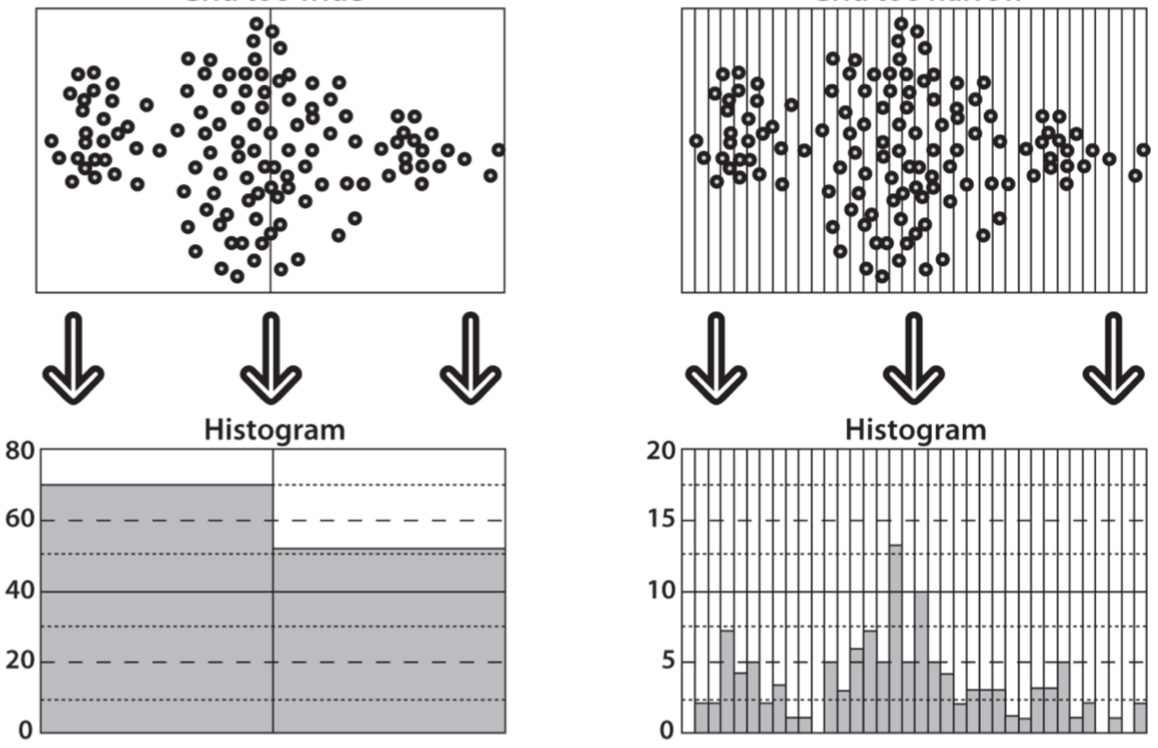
\includegraphics[width=0.80\textwidth]{figures/histogram_bin_size.png}}
\caption{\label{fig:histogram-bin-size}If the range of the bins is too large, then the distribution is coarse (left). If the range of the bins is too small, then the distribution is not accurately represented and spikes cells appear (right). Image courtesy of Bradski and Kaehler.}
\end{figure}

One of the inaccuracies with colour histograms lies within the scope of the distribution. If the histogram represents the global distribution of all the pixels in the still, then two images might have very similar histograms \cite{petkovic2000}. For example, a histogram containing 60\% white pixels and 40\% blue pixels could either describe both a blue sky with white clouds, or a snowy landscape with a blue sky. Despite both histograms being good colour-based features, the actual result is still poor when it will be used for matching the histograms. A solution consists in segmenting the still into multiple local images, and extract the local colour-based features for each segment. For example, the still could be partitioned into a 5x5 grid, and a colour histogram could then be computed for each grid \cite{yan2007review}. This would enable colour-based features to represent specific regions of the still rather than globally describing an image. However, the same problem mentioned earlier could occur if the still is segmented into too many regions, causing the overall histogram to be coarse.\\

Other types of colour-based features can be extracted from images and videos such as colour moments, colour correlograms \cite{huang1997correlograms} and Gaussian models. However, colour-based features have their limitations as they cannot describe textures and shapes, rendering them inefficient in certain applications \cite{hu2011survey}.

\subsubsection{Texture-based Features}

Texture-based features are often used in parallel with colour-based features. The aforesaid problem where two different objects might share a similar histogram e.g. green tree leaves and green grass, can be solved by using texture-based features to differentiate them. These can be differentiated by using a variety of features such as Tamura features, which extract information including coarseness, contrast, and directionality of the objects \cite{amir2003ibm}. 

\subsubsection{Shape-based Features}

Shape-based features are used to describe the overall shape of objects present in the image. The most common approach consists in computing a EHD\footnote{Edge Histogram Descriptor}, which consists in detecting the edges present in the image (see Section edges) and then plot their spatial distribution in an histogram by counting the number of pixels for each edge \cite{hauptmann2004informedia}. The same image segmentation technique can be used to localise the EHD. These shape-based features have many applications, but are harder to extract and require more computing power than colour-based features and texture-based features.

% ----------------------------------------------------

\subsection{Dynamic Features}
\label{sec:dynamic-features}

In contrast to static features, which can be extracted from individual video frames, dynamic features require the continuity between consecutive frames to extract relevant visual descriptors, making use of the temporal aspect of the video mentioned in section \ref{sec:temporal-aspect-videos}). These features can be divided into two subcategories: object features and motion features. However, before reviewing the techniques used to extract these features, it is important to specify what defines a good visual feature.

\subsubsection{Corner Detection}

Figure \ref{fig:monaco_palace_features} shows an image with coloured windows used to make the difference between poor and good potential features that could be used for object and motion features:
\begin{itemize}
	\item \textit{Flat surfaces} are portrayed in blue in Figure \ref{fig:monaco_palace_features}. These blue windows are spread over large areas of the image, meaning it is difficult to find their specific location. Moving the blue window along the image in any direction will result in the same visual content being represented in the window. Therefore, these flat regions are the worst structures as they do not contain any useful information.
	\item \textit{Edges} are characterised in green in Figure \ref{fig:monaco_palace_features}. These are more informative than flat surfaces as they can be more accurately localised, but pinpointing an exact location is still hard as the patch can be moved in the direction parallel to the edge's. Moving the green window along the edge will again result in the same visual content being represented in the window. Edges are efficient to detect object boundaries, but not for tracking specific points.
	\item \textit{Corner} are characterised in red in Figure \ref{fig:monaco_palace_features}. These are the most descriptive points as they are often unique and can be precisely located in an image. Moving the red window in any direction will cause it to look different. Corners are therefore the ideal candidate for features used in object matching and tracking.
\end{itemize}

\begin{figure}[h] 
\centerline{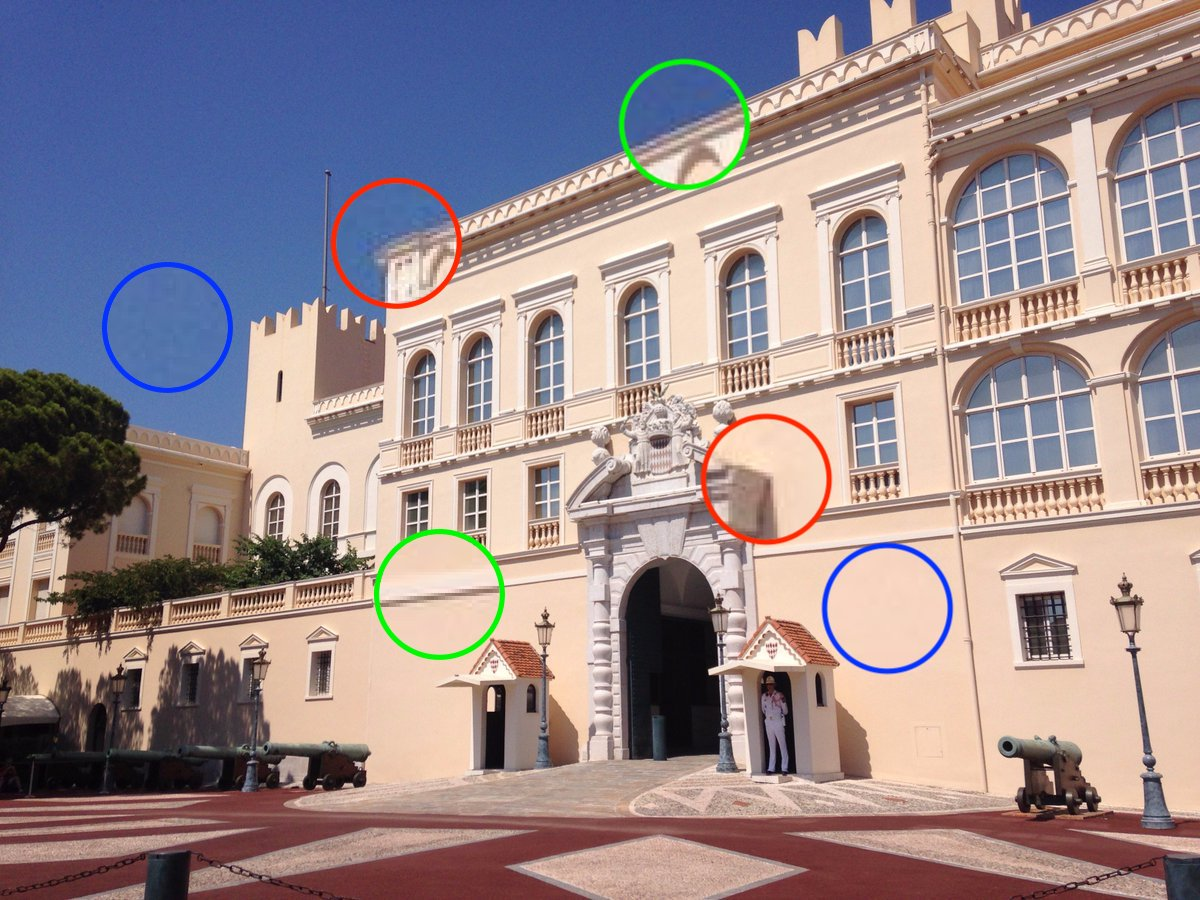
\includegraphics[width=0.75\textwidth]{figures/monaco_palace_features.jpg}}
\caption{\label{fig:monaco_palace_features}An image of the Palace of Monaco with coloured windows representing poor features in blue (flat), edges in green, and good features in red (corners).}
\end{figure}

Once expressive and unique descriptors like corners are detected, they can be used to extract object features and motion features, and to compute similarities between the query video and the videos in the database.\\

Many different techniques exist to find robust features and interest points: Harris Corner Detection, SIFT, SURF.

\begin{comment}
    detect edges and then use that to detect corners
\end{comment}

\subsubsection{Object Features}

Object features correspond to objects that are detected using the colour, texture and size of image regions. Some of the most common objects usually detected in videos are faces, as many CBVR systems use them to compute similarities between videos \cite{sivic2005face}. However, extracting object features is time-consuming and expensive in terms of required processing power, which is why CBVR algorithms either focus on detecting specific sets of objects rather than general objects that may be present in a scene, or on static features.

\subsubsection{Motion Features}

camera-based motion features

object-based motion features

Example algorithms: optical flow (Dense Optical Flow, Farneback Polynomial Expression Algorithms, Lucas-Kanade Algorithm.
Can calculate optical flow to prune camera movement caused by unstable recording e.g. hand shaking movement \cite{wang2016actionregonition}.


%%%%%%%%%%%%%%%%%%%%%%%%%%%%%%%%%%%%%%%%%%%%%%%%%%%%%%%%%%%%%%%%%%%%%%%%%%%%%%%%%%
% 3 - LEARNING MODELS FOR FEATURE MATCHING
%%%%%%%%%%%%%%%%%%%%%%%%%%%%%%%%%%%%%%%%%%%%%%%%%%%%%%%%%%%%%%%%%%%%%%%%%%%%%%%%%%
\section{Learning Models for Classification}

Multiple techniques exist to retrieve a video's visual information to later compare it to the visual information stored in the database.
Retrace evolution of pattern matching methods: BoW to CNN (and before? --> find surveys)

% ----------------------------------------------------

\subsection{Bag-of-Visual-Words}

\subsubsection{BoW}
BoW for documents

\subsubsection{BoVW}

BoVW

TODO:
\begin{itemize}
    \item Explain how Bag-of-Words model works
    \item H. Wang's implementation of BoW histogram \cite{wang2016actionregonition}
    \item State that Fisher Vectors are an improvement on BoW
\end{itemize}

\subsubsection{Histogram Comparison}

chi-square
alternative chi-square
intersection
bhattacharyya

% ----------------------------------------------------

\subsection{Deep Learning}

\subsubsection{Classical Neural Networks}

nn

\subsubsection{Convolutional Neural Networks}

cnn


%%%%%%%%%%%%%%%%%%%%%%%%%%%%%%%%%%%%%%%%%%%%%%%%%%%%%%%%%%%%%%%%%%%%%%%%%%%%%%%%%%
% 4 - STRUCTURAL MOVIE PRE-PROCESSING
%%%%%%%%%%%%%%%%%%%%%%%%%%%%%%%%%%%%%%%%%%%%%%%%%%%%%%%%%%%%%%%%%%%%%%%%%%%%%%%%%%
\section{Structural Movie Pre-Processing}

The database of videos can be pre-processed to optimise the visual content extraction and pattern matching phases. As stated in Section \ref{sec:temporal-aspect-videos} on the temporal aspects of videos, movies can be defined as a logically ordered collection of scenes, which may contain different shots, all made up of individual frames. Pre-processing the database of movies by segmenting it into a list of shots and representing each shot with a single key frame is a profitable solution that will exponentially improve a CBVR system's efficiency. However, a limit must be set on the amount of data that is segmented to balance the efficiency and the accuracy of the CBVR system.

% ----------------------------------------------------

\subsection{Temporal Movie Segmentation}

The frames that make up a shot usually show strong content correlation. This means that features extracted from one frame will be extremely similar in another frame from the same shot. Detecting shot boundaries would allow the movie to be segmented and organised by shots, as depicted in Figure \ref{fig:shot_boundary_detection}. These boundaries are defined by the type of transition between two different shots, which can either be defined as a quick cut when the transition is direct, or as gradual when it is a dissolve or fade in/out transition \cite{yuan2007shotboundary}, as shown in Figure \ref{fig:video_transitions}.

\begin{figure}[h] 
\centerline{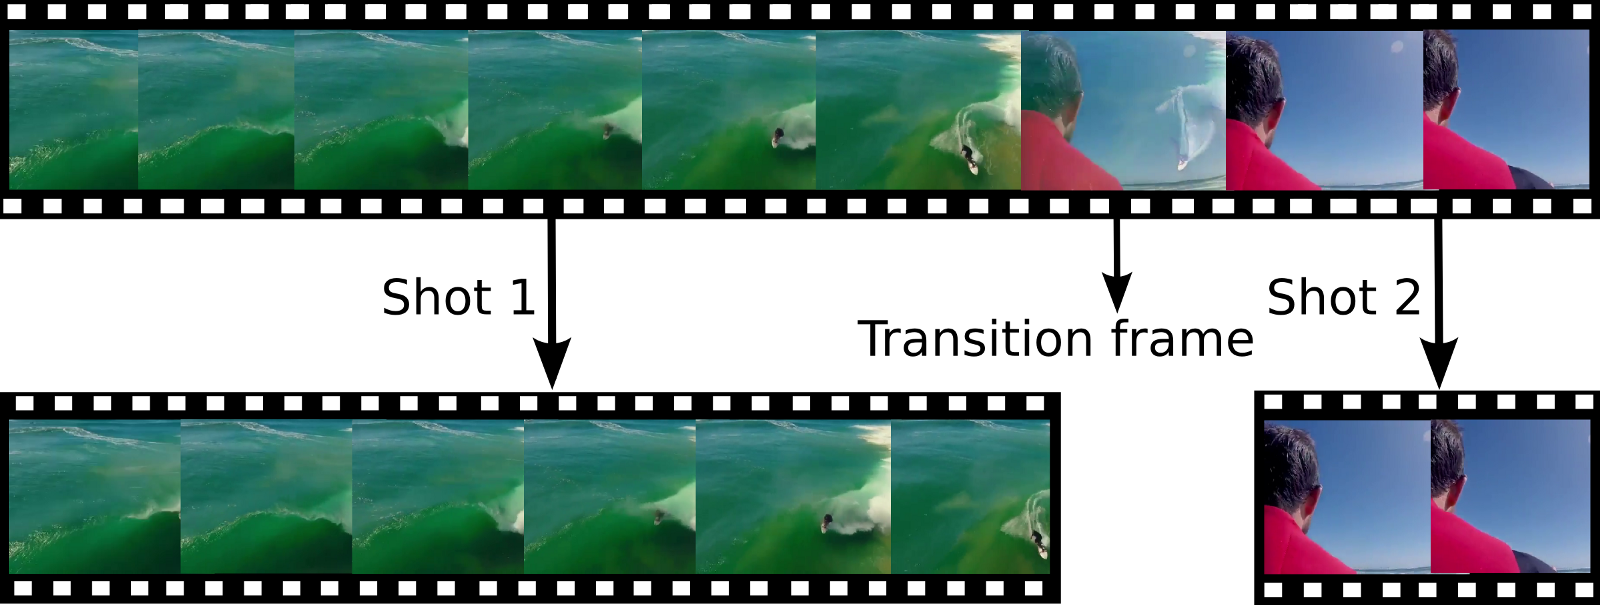
\includegraphics[width=0.75\textwidth]{figures/shot_boundary_detection.png}}
\caption{\label{fig:shot_boundary_detection}Shot boundary detection example of a video made up of two shots with a gradual transition. Figure courtesy of Michael Gygli available online at: \url{https://medium.com/gifs-ai/\_ridiculously-fast-shot-boundary-detection-with-fully-convoluti\_onal-neural-networks-da9d8c73e86c}}
\end{figure}

\begin{figure}[h] 
\centerline{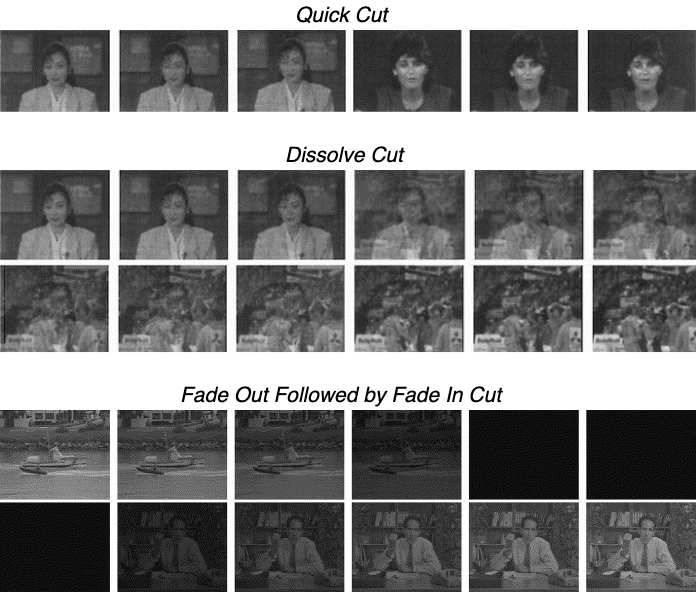
\includegraphics[width=0.75\textwidth]{figures/video_transitions.png}}
\caption{\label{fig:video_transitions}. Visual examples of a quick cut, a dissolve cut and a fading cut. Frames courtesy of (Koprinska, Carrato, 2001) ``Temporal video segmentation: A survey'' available online at: \url{https://www.sciencedirect.com/science/article/pii/S0923596500000114}}
\end{figure}

Temporal video segmentation requires three steps:
\begin{enumerate}
    \item feature extraction
    \item similarity measurements
    \item shot boundary detection
\end{enumerate}

\subsubsection{Feature Extraction}
The first step in video segmentation consists in extracting features. These features include all the diverse types mentioned in Section \ref{sec:visual-content-extraction}, ranging from static features such as colour-based features (e.g. colour histograms) to dynamic features such as corner points and SIFT\footnote{Scale Invariant Feature Transform}. Although colour histograms are simple to compute and work well with most shots as long as there is at most minor camera movement, they are inefficient when the shots contain major camera movements. For example, if in the shot the camera moves from the inside a house towards the outside by going through the window, the frames retrieved from the beginning of the shot will be extremely different to frames from the end of the shot.\\

Dynamic features are therefore more efficient for shot boundary detection than histograms due to their robustness. On the one hand, edge features are more vigorous than histograms when dealing with major camera movement and can handle changes in luminosity. On the other hand, corner and motion features can additionally handle camera motion and the impact of objects in the shot such rapid motion e.g. people walking in front of the camera. However, these dynamic features are much more complicated to extract and do not always outperform colour histograms. Due to their simplicity, colour histograms remain the most common feature extraction technique for shot boundary detection.\\

\subsubsection{Similarity Measurements}
The second step in video segmentation is to use these extracted features to compute the similarities between frames. Many metrics exist to compute the similarities between two the extracted features. The most basic method consists in computing the Euclidean distance between features. More advanced methods can be used based on the type of feature that was extracted. For instance, histogram intersection and chi-square similarity can be used to compute the relationship between colour histograms. During the 2006 TRECVID conference, \cite[p.2]{hoi2006trecvid06} used gray scale histograms for their extracted features and calculated the colour differences between frames using the EMD\footnote{Earth Mover's Distance}. EMD is used to calculate the distance between two probability distributions, which are represented by the two histograms that represent each frame in \cite{hoi2006trecvid06}'s case. These similarities can be measured using two techniques.\\

The first technique rests on using pairs of frames to compute the similarities between them. The similarities between two consecutive frames $I_1$ and $I_2$ are compared, before comparing the pair of frames $I_2$ and $I_3$, and so on and so forth until frames $I_{n-1}$ and $I_n$ are compared. This straightforward technique easily detects rough changes between the visual content in a shot, such as quick cuts between two shots, but is more susceptible to noise and disturbance.\\

The second technique is the window-based similarity measure, that measures the similarities between multiple frames specified within a range. This helps counter the effects of noise and disturbances captured by the pair-based approach but is more expensive to compute, therefore less used.

\subsubsection{Detection}
The final step in segmenting a video is the detection of the frames to cut, which is achieved by using the measured similarities between the frames. Two methods exist for this step: a threshold-based approach and a statistical learning-based approach.\\

The threshold-based approach compares the measured similarities between a pair of frames with a threshold. Whenever the similarity measure is smaller than the threshold, a shot boundary is detected and the shot can be cut. Figure \ref{fig:shot_boundary_detection_threshold} betrays an example of a threshold-based approach for different types of transitions, with a correct detection (\emph{A}), a missed detection (\emph{B}) and a misinterpreted detection (\emph{C}).\\

\begin{figure}[h] 
\centerline{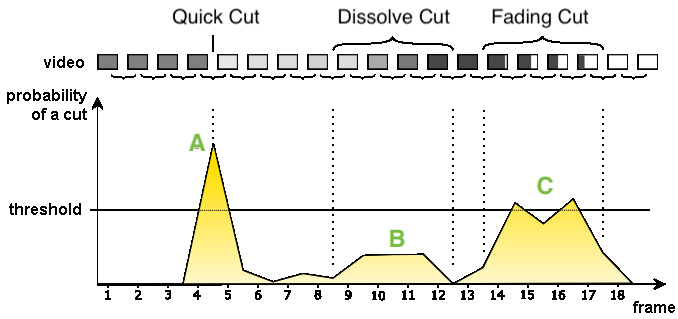
\includegraphics[width=0.75\textwidth]{figures/shot_boundary_detection_threshold.png}}
\caption{\label{fig:shot_boundary_detection_threshold}Threshold-based approach for shot boundary detection. In this example, the shot boundary is detected at \emph{A}, it is missed at \emph{B}, and it is misinterpreted at \emph{C} as two cuts rather than a single one.}
\end{figure}

Either global thresholds, adaptive thresholds, or combinations of both can be used:
\begin{itemize}
    \item \textit{Global thresholds} are set empirically and predefined for the entire video. They are therefore inefficient when trying to detect local variations as these are not integrated into the initial global threshold calculations.
    \item \textit{Adaptive thresholds} are local thresholds that are continuously calculated for windows of frames. As the window slides across the video, the threshold is re-estimated accordingly to account for local variations. These are more accurate than global thresholds but are harder to estimate and require some knowledge about the video to set variables such as the window's size.
    \item \textit{Combination of global and adaptive thresholds} are adaptive thresholds that take into account the values of global thresholds when estimating the frames within the window. Different thresholds can be determined for different types of transitions such as cut and dissolve transitions. However, these add additional complexity to the threshold estimation.
\end{itemize}

The statistical learning-based approach is two-class classification task where each frame is classified either as a ``shot change`` or as a ``no shot change`` based on the extracted features and the similarity measurements between those features. Two types of classifiers can be used for this approach:
\begin{itemize}
    \item \textit{Supervised learning-based classifiers}, such as the SVM\footnote{Support Vector Machine} and Adaboost. These supervised learning approaches have multiple advantages compared to threshold-based approaches as they do not require thresholds to be set and many different types of features can be combined in the feature extraction step to increase the classifier's accuracy. However, this approach requires more expertise as the classifier relies on a well-trained data set to remain accurate.
    \item \textit{Unsupervised learning-based classifiers} are divided into frame similarity-based and frame-based algorithms. \textit{Frame similarity-based classifiers} groups the similarity measurements between a pair of frames into two clusters. The first cluster holds the similarity measurements with low values, which correspond to the ``shot change'' class, while the second cluster holds the similarity measurements with high values, which correspond to the ``no shot change'' class. Alternatively, \textit{frame-based classifiers} consider each shot as a cluster of frames with similar features. The advantage of unsupervised learning-based classifiers over supervised ones is that no training is required, but the logical temporal order of the shots in scenes is not preserved.
\end{itemize}

All the aforementioned techniques in this section that are used in the three steps required in the process of segmenting a video can be applied to feature-length movies but require some improvements to work efficiently with these large videos. For instance, \cite{hanjalic1999moviesegmentation} suggests considering the semantic aspects of movies, since people relate to the story, such as a marking dialogue, when they remember a movie.

% ----------------------------------------------------

\subsection{Key Frame and Thumbnail Extraction}

\subsubsection{Key Frames}

Y. S. Heo et al. \cite{heo2016colortransfer} suggests only considering key frames in videos to operate on. These key frames would be used for the feature extraction, database pre-processing and pattern matching phases. Key frames are determined based on the difference between two consecutive frames using the histogram chi-square distribution approach (See Equation \ref{eq:chisquare}).\\

\cite{heo2016colortransfer}
This approach only considers key frames from the query video clip. Key frames are determined based on the difference between two consecutive frames using the histogram chi-square distribution approach (See Equation \ref{eq:chisquare}).\\

TODO:
\begin{itemize}
    \item Explain histogram chi square distribution technique.
    \item When the amount of differences $\theta$ between two frames exceeds a threshold, usually set at the empirical value $\theta = 0.005$, then the current frame is set as a key frame.
\end{itemize}

\begingroup \Large \begin{equation} \label{eq:chisquare}
    C(h^{t-1}, h^{t}) = \sum_{i=0}^{255} \frac{(h_{i}^{t-1} - h_{i}^{t})^2}{h_{i}^{t-1} + h_{i}^{t}}
\end{equation} \endgroup \\

To illustrate the advantage of using key frames, let's use a 3-seconds long shot recorded at 30 fps\footnote{Frames Per Second} of a ball rolling on the ground, which would consist of a total of 90 frames. Analysing all the frames individually as stills would be highly inefficient. However, selecting key frames to work on, as depicted in Figure \ref{fig:rolling_ball} where a single frame is chosen for each second, would means that 3 key frames can be used for feature extraction and pattern matching instead of using all of the 90 frames that make up the video.\\

\begin{figure}[h]
\centerline{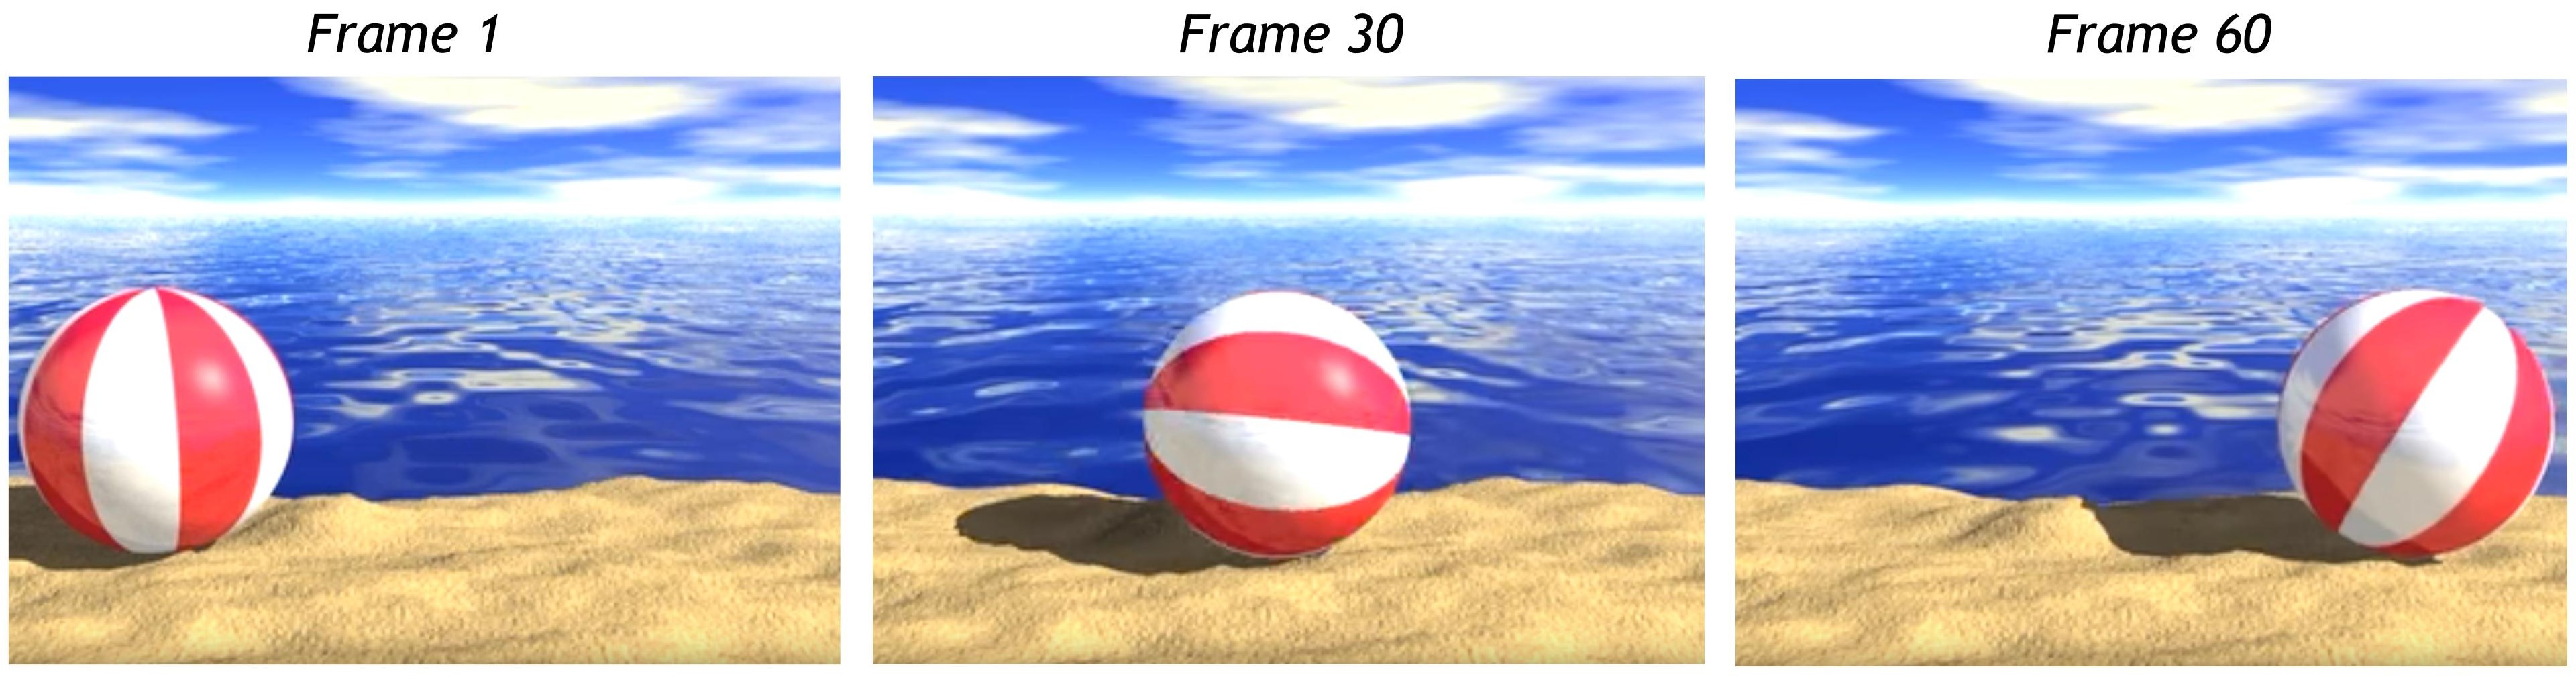
\includegraphics[width=\textwidth]{figures/ball_rolling.jpg}}
\caption{\label{fig:rolling_ball}Example of frames to sample for low-visual content analysis. The first frame for each second (one frame every thirty seconds) is retrieved for a 30 fps 3-second video of a ball rolling from the left-hand side of the screen to the right-hand side. Video frames courtesy of \textit{``How to Animate a Rolling Ball"} YouTube video available online: \url{https://youtu.be/cgbLAreElNI?t=130}.}
\end{figure}

\subsubsection{Thumbnails for Initial Shortlisting}

In their work, M. Okabe et al. \cite{okabe2018animating} generate thumbnails for each video in their database, which are stored as additional data along with the original video file. The thumbnails for the query video and for the database videos would be generated using the same algorithm in order to create similar results. This technique can be used in parallel to A. Araujo et al.'s \cite{araujo2017i2v}, who states that an initial shortlist of potentially matching videos can be generated before the main pattern matching phase. This shortlist can be created by computing the similarities between the query video's thumbnail and the thumbnails of the database videos.\\

Many advantages can be gained from this small initial step which could have an important impact on the system's overall speed and efficiency performance. Indeed, database videos that share no similarities to the query video will not be considered at all during the main pattern matching phase e.g. if the query video corresponds to a colourful sunset, then database videos of cloudy environments will be immediately filtered out as it is unlikely that they will match with the query video in the main pattern matching phase. This step diminishes the number of the videos to compare to the query.\\

This initial step is extremely speedy as it only uses a single frame that describes the entire video. Therefore the entire process will not be noticeably slowed down. However this concept could only be applied on relatively small databases where the videos contain a single scene with multiple similar shots. Indeed, shots can be characterised by a single still as they are made up of frames with similar visual content, whereas scenes can be made up of shots that change a lot and describe different visual content. Using thumbnails to shortlist a database of feature-length movies would greatly diminish the accuracy of the system due to the high number of scenes that make up a movie that cannot be resumed to a single thumbnail. The database videos' thumbnails will have already been generated during the database's pre-processing phase, which only occurs a single time. A possible solution could be to create a thumbnail for each shot in a scene, and store each thumbnail in a list. For example, if a scene contains six different shots, then six thumbnails will be generated to describe that scene.\\

\begin{comment}
\cite{okabe2018animating}
For quicker pattern matching and feature extraction, 16 pixels separate two feature points, allowing for rough pattern matching rather than exact pattern matching. This could be used when using feature-length movies as database videos to pattern match.
\end{comment}

% ----------------------------------------------------

\subsection{Fisher Vectors}

TODO:
\begin{itemize}
    \item Fisher Vectors can be used to generate a compact signature for videos, which will then be used for computing similarities between the query video's FV and the database videos' FVs \cite{araujo2017i2v}
\end{itemize}


%%%%%%%%%%%%%%%%%%%%%%%%%%%%%%%%%%%%%%%%%%%%%%%%%%%%%%%%%%%%%%%%%%%%%%%%%%%%%%%%%%
% 5 - CHAPTER SUMMARY
%%%%%%%%%%%%%%%%%%%%%%%%%%%%%%%%%%%%%%%%%%%%%%%%%%%%%%%%%%%%%%%%%%%%%%%%%%%%%%%%%%
\section{Chapter Summary}

chapter summary

% \chapter{Requirements}
% If you are doing a primarily software development project, this is the
% chapter in which you review the requirements decisions and
% critique the requirements process.

% \chapter{Design}
% This is the chapter in which you review your design decisions at various
% levels and critique the design process.

% \chapter{Implementation and Testing}
% This is the chapter in which you review the implementation and testing
% decisions and issues, and critique these processes.

% Code can be output inline using \verb@\lstinline|some code|@.  For example,
% this code is inline: \lstinline|public static int example = 0;|  (I have
% used the character \verb@|@ as a delimiter, but any non-reserved character
% not in the code text can be used.)

% Code snippets can be output using the \verb|\begin{lstlisting} ... \end{lstlisting}|
% environment with the code given in the environment.  For
% example, consider listing \ref{Example-Code}, below.

% \begin{lstlisting}[breaklines,breakatwhitespace,caption={Example code},label=Example-Code]
% public static void main() {

%   System.out.println("Hello World");

% }
% \end{lstlisting}

% Code listings are produced using the package ``Listings''.  This has many
% useful options, so have a look at the package documentation for further
% ideas.

% \chapter{Results}
% This is the chapter in which you review the outcomes, and
% critique the outcomes process.  You may include user evaluation here
% too.

% \chapter{Conclusions}
%This is the chapter in which you review the major achievements in the
light of your original objectives, critique the process, critique your
own learning and identify possible future work.

This is the chapter in which you review the major achievements in the
light of your original objectives, critique the process, critique your
own learning and identify possible future work.


\bibliography{Bibliography}

% \appendix

% \chapter{Design Diagrams}

% \chapter{User Documentation}

% \chapter{Raw results output}

\end{document}